\documentclass[14pt, a4paper]{extarticle}
\usepackage{amsmath}
\usepackage{amssymb}
\usepackage{mathtools}
\usepackage{mathtext}
\usepackage[T1, T2A]{fontenc}
\usepackage[utf8]{inputenc}
\usepackage[english, russian]{babel}
\usepackage{cmap}
\usepackage{fancyhdr}
\usepackage[pdftex]{graphicx}
\usepackage{gensymb}
\usepackage{floatrow}
\usepackage{titlesec}
\usepackage{lastpage}
\usepackage{float}
\usepackage{gensymb}
\usepackage{booktabs}
\usepackage{mathrsfs}
\usepackage{floatflt}
\usepackage{wrapfig}
\usepackage{caption}
\usepackage{ upgreek }

\graphicspath{{pictures/}}
\DeclareGraphicsExtensions{.pdf,.png,.jpg}
\newtheorem{task}{Задача}
\begin{document}
\selectlanguage{russian}


\begin{titlepage}
\begin{center}

\textsc{\LARGE Московский\\[-0.2cm]Физико-Технический Институт\\[0.1cm]\large (национальный исследовательский университет)}\\[1.5cm] 


\includegraphics[width=0.3\textwidth]{logo}

\textsc{\Large Лабораторная работа 5.10.1: \\ }

% Title
\HRule \\[0.4cm]
{ \LARGE \bfseries Электронный парамагнитный резонанс }

\HRule \\[1.5cm]

% Author and supervisor
\noindent
\begin{minipage}{0.4\textwidth}
\begin{flushleft} \large
\end{flushleft}
\end{minipage}%
\begin{minipage}{0.4\textwidth}
\begin{flushright} \large
\end{flushright}
\end{minipage}

\large{\begin{flushright}
\vfill
\textbf{Выполнил}:\\
\textbf{Маслюк Руслан\\}
\textbf{группа Б05-871}
\end{flushright}}

{\large \today}\\

\end{center}
\end{titlepage}

\section{Цель}
\label{sec:цель}
Исследовать электронный парамагнитный резонанс в молекуле ДФПГ, определить g - фактор электрона, измерить ширину линии ЭПР.
\section{Вступление}
\subsection{Теория}
Энергетический уровень электрона в присутствии магнитного поля $B$ расщепляется
на два подуровня. Расстояние между ними равно
\begin{equation}
    \label{eq:(1)}
    \Delta E = E_2 - E_1 = 2 \mu B
\end{equation}
Между уровнями возможны переходы. Они могут возбуждаться внешним высокочастотным
магнитным полем. Резонансное значение частоты определяется из соотношения
\begin{equation}
    \label{eq:(2)}
    \hbar \omega_0 = \Delta E = 2 \mu B
\end{equation}
При переходе с нижнего на верхний уровень квант энергии поглощается, а при
обратном переходе излучается квант той же частоты. Возбуждение электронных
резонансных переходов ЭМ полем с частотой $\omega_0$ называется электронным
парамагнитным резонансом.
\\
Без внешнего высокочастотного поля заселенность верхнего и нижнего уровней $N_u$
и $N_d$ определяется температурой и описывается формулой Больцмана
\begin{equation}
    \label{eq:(3)}
    \frac{N_u}{N_d} = \exp \left( - \frac{\Delta E}{k T} \right)
\end{equation}
Гиромагнитное соотношение
\begin{equation}
    \label{eq:(4)}
    \mu = \gamma \vec{M}
\end{equation}
Если магнитный момент выражается в магнетонах Бора, а механический в единицах
$\hbar$, то связь выражается через фактор Ланде
\begin{equation}
    \label{eq:(5)}
    \frac{\mu}{\mu_B} = \frac{g \vec{M}}{\hbar}
\end{equation}
Можно выразить $g$-фактор через определяемые экспериментально величины
\begin{equation}
    \label{eq:(6)}
    g = \frac{\hbar \omega_0}{\mu_B B}
\end{equation}

\subsection{Оборудование} % (fold)
\label{sec:оборудование}
Для наблюдения электронного парамагнитного резонанса необходимы чувствительные радиоспектроскопы. В нашей работе используется радиоспектроскоп несложной конструкции, обладающий достаточной чувствительностью, чтобы уверенно наблюдать электронный парамагнитный резонанс на ДФПГ. 
Схема радиоспектроскопа изображена на рис. 1. Основной частью радиоспектроскопа является колебательный контур.
\begin{figure}[h!]
	\centering
	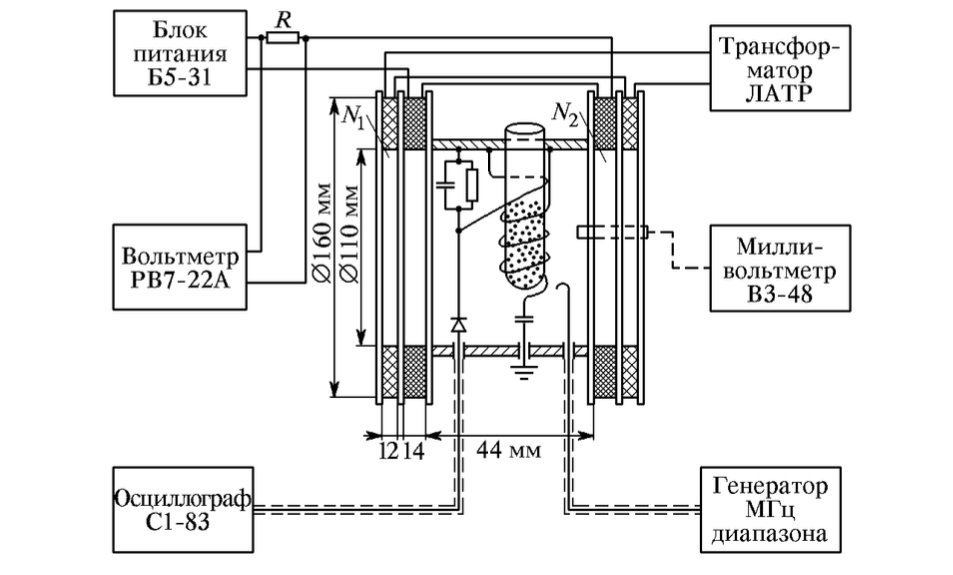
\includegraphics[width = 0.4\paperwidth]{laba_10_1_scheme}
	\caption{Блок-схема установки для налюдения ЭПР. Измерение постоянного и переменного токов через катушки $N_2$ производится с помощью вольтметра РВ7-22А и сопротивления R = 10 Ом, включенного в цепь катушек}
\end{figure}
Он состоит из катушки индуктивности и плоского конденсатора. Контур заключен в латунный посеребренный изнутри контейнер. Ампула с исследуемым образцом вставляется в катушку индуктивности контура. Основное магнитное поле в образце создается с помощью двух соосно расположенных катушек, питаемых от источника постоянного тока. 
\clearpage


\section{Ход работы} % (fold)
\label{sec:ход_работы}
Настроим генератор на резонансную частоту контура, включим питание основных катушек, и плавно меняя реостатом величину тока, проходящего через основные катушкаи найдем сигнал электронного парамагнитного резонанса.
$f_{res} = 126,76\pm 0,02 МГц$\\
$f_h = 126,49 \pm 0,02 МГц$\\
$f_l = 126,49 \pm 0,02 МГц$, тогда Добротность контура:\\
$$
Q = \frac{f}{\Delta f} = \frac{f_{res}}{f_h - f_l} = \frac{126,76}{0,48}\approx264,1
$$ 
$$
\varepsilon_Q = \varepsilon_{f_{res}} + \varepsilon_{\Delta f} = 0,08
$$
$$
\sigma_Q = 21,
$$Тогда
$$
Q = (2,6\pm0.2)\cdot10^2
$$
Определим g-фактор электрона, для этого найдем резонансные значениязначения частоты $\omega_0 $ и индукции $B_0$. Для этого воспользуемся более маленькой катушкой с N = 45, $d = 15,2\pm 0,1$мм
Зная также ЭДС $\varepsilon_i = (2,51\pm0,01)\cdot10^{-3}В$ и частоту $\nu = 50 Гц$, найдем величину модулирующего поля:
$$B=\sqrt{2} \frac{2 \varepsilon_i}{\pi^2d^2N\nu} \approx 1,52 \cdot 10^{-3}Тл = 1,52 \text{мТл}$$
$$\varepsilon_B = \varepsilon_{\varepsilon_i} + 2\varepsilon_d = 0,003 + 0,013
= 0,016$$
$$\sigma_B = 0,024 \text{мТл}$$
$$B = 1,52 \pm 0,024 \text{мТл}$$
Для полуширины на полувысоте линии резонансного поглощения получим
$$\Delta B= \frac{A_{half}}{A_{full}} B = 0,146 \text{мТл}$$
Калибровочный график (напряжение на пробной катушке от внешнего):
\begin{figure}[h!]
	\centering
	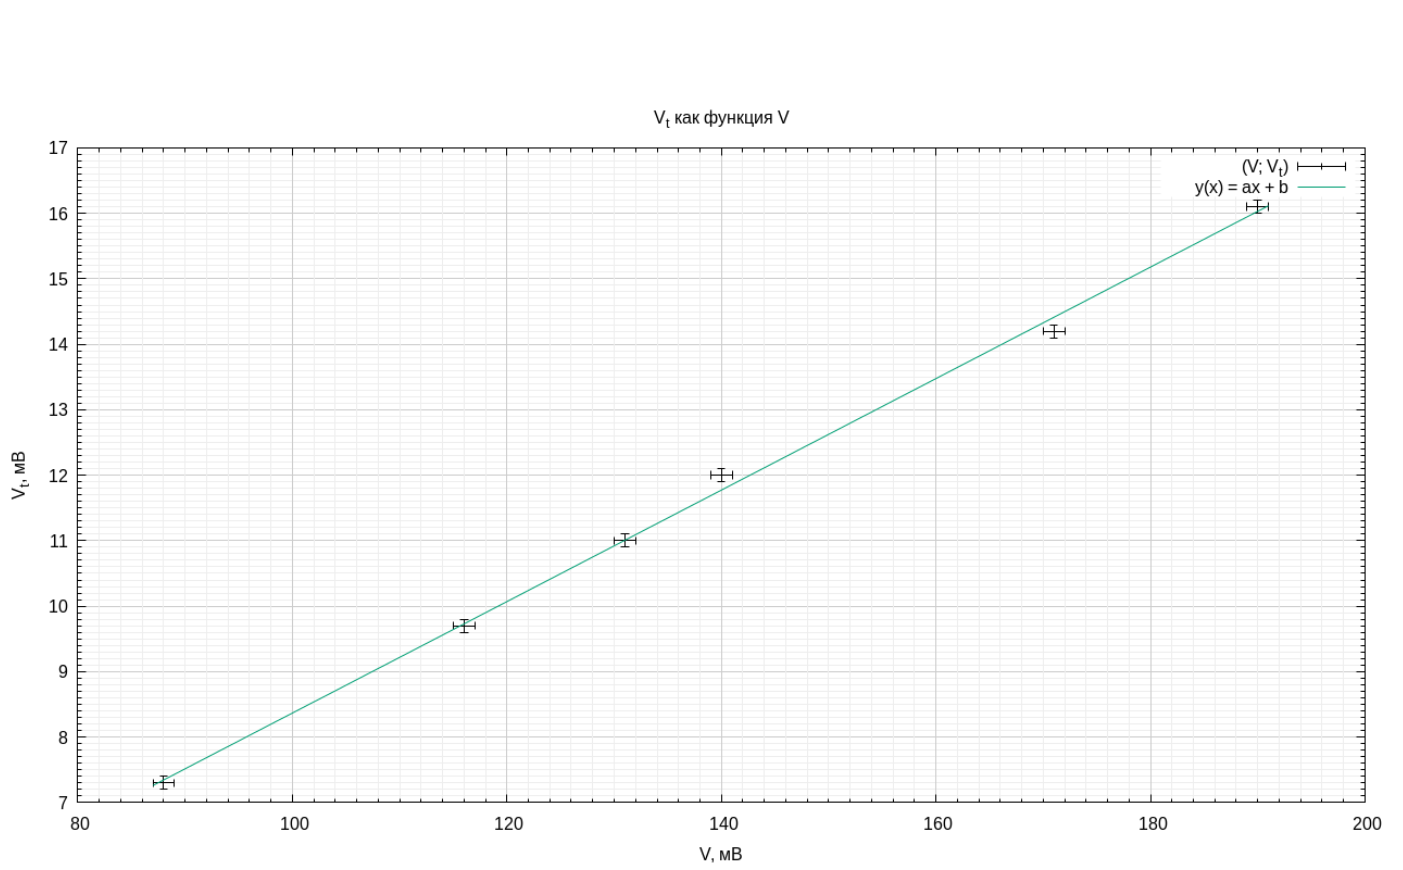
\includegraphics[width = 0.7\linewidth]{graph_1}
	\caption{Калибровочный график}
\end{figure}
$$B_0=\frac{V_t}{NS 2 \pi \nu} = 7,03 \pm 0,45 \text{мТл}$$
Тогда
$$g = 1,9 \pm 0,2$$
График зависимости резонансной частоты от силы тока:
\begin{figure}[h!]
	\centering
	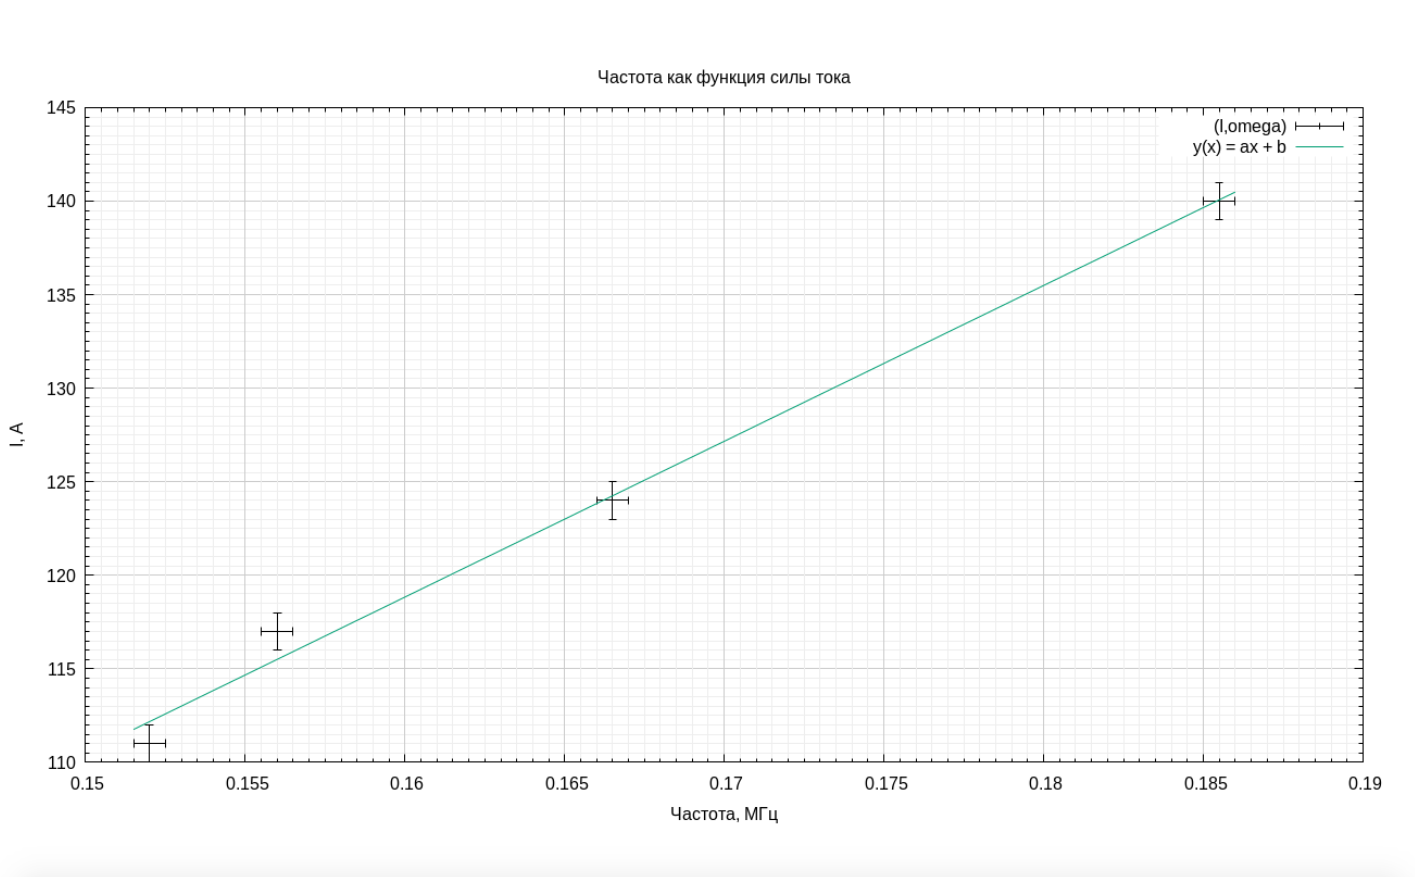
\includegraphics[width = 0.7\linewidth]{graph_2}
	\caption{График зависимости резонансной частоты от силы тока}
\end{figure}
% section ход_работы (end)
\section{Результаты} % (fold)
\label{sec:результаты}
Выполнив данную лабораторную работу, мы измерили $g$-фактор электрона,
пронаблюдав явление ЭПР. Он оказался равен $g = 1,9 \pm 0,2$, что совпадает с табличным значением.
% section результаты (end)
\section{Вывод} % (fold)
\label{sec:вывод}
Мы Исследовали электронный парамагнитный резонанс в молекуле ДФПГ, определили g - фактор электрона, измерили ширину линии ЭПР. И g - фактор совпал с табличным значением.
% section вывод (end)
\end{document}